\documentclass[11pt, oneside]{article}   	% use "amsart" instead of "article" for AMSLaTeX format
\usepackage{geometry}                		% See geometry.pdf to learn the layout options. There are lots.
\geometry{letterpaper}                   		% ... or a4paper or a5paper or ... 
%\geometry{landscape}                		% Activate for for rotated page geometry
%\usepackage[parfill]{parskip}    		% Activate to begin paragraphs with an empty line rather than an indent
\usepackage{graphicx}				% Use pdf, png, jpg, or eps� with pdflatex; use eps in DVI mode
								% TeX will automatically convert eps --> pdf in pdflatex		
\usepackage{amssymb}
\usepackage{amsmath}
\usepackage{parskip}

\title{Integration---practice problems}
%\author{The Author}
%\section{}
% \subsection*{R code}
\date{}							% Activate to display a given date or no date

\graphicspath{{/Users/telliott_admin/Dropbox/Tex/png/}}

\begin{document}
\maketitle
\Large
%\noindent
We can construct some good problems of our own, looking at what we get by differentiating various products, using the "product rule".  The first one is particularly enlightening.

\[ \frac{d}{dx} \ \sin x \cos x  = (\sin x \cos x)' \]
\[ = \sin x \cos x' + \sin x' \cos x \]
\[ = -\sin^2 x + \cos^2 x \]
Starting with the identity $\sin^2 x + \cos^2 x = 1$, we can rearrange to obtain:
\[ \sin^2 x + \cos^2 x - 1 = 0 \]
\[ -\sin^2 x - \cos^2 x + 1 = 0 \]
Using these, the derivative above can be rearranged in various ways (by addition of the second identity):
\[  \frac{d}{dx} \ \sin x \cos x  = 1 - 2 \sin^2 x \]
and (by addition of the first identity):
\[   \frac{d}{dx} \ \sin x \cos x  = 2 \cos^2 x - 1  \]
A third  way uses the formula for addition of cosines:
\[ \cos(s+t) = \cos s \cos t - \sin s \sin t \]
\[ \cos 2s = \cos^2 s - \sin^2 s = 2 \cos^2 s - 1 \]
Thus, a third version of the derivative is
\[ (\sin x \cos x)' =  \cos 2x \]
Summarizing, the equivalent forms are:
\[ (\sin x \cos x)' =  1 - 2 \sin^2 x \]
\[ = 2 \cos^2 x - 1 \]
\[ =  \cos 2x \]

Using the second version 
\[ \sin x \cos x)'  = 2 \cos^2 x - 1 \]
and integrating
\[ \int \ ( \sin x \cos x)' \ dx = \int 2 \cos^2 x \ dx -  \int 1 \ dx   \]
\[ \sin x \cos x = 2 \int \cos^2 x \ dx - x \]
\[ \int cos^2 x \ dx = \frac{1}{2} \ [ \ x + \sin x \cos x \ ]  + C \]

And since (by the addition formula for sine)
\[ \sin(s + t) = \sin s  \cos t + \cos s \sin t  \]
if $s=t$ then
\[ \sin 2s = 2 \sin s \cos s \]
\[ \frac{1}{2} \sin 2s = \sin s \cos s \]

Plugging in above
\[ \int cos^2 x \ dx = \frac{1}{2} \ [ \ x + \sin x \cos x \ ] \]
\[ = \frac{1}{2} \ [ \ x + \frac{1}{2} \sin 2x \ ] \]

On the other hand, above we had
\[  (\sin x \cos x)' =   \cos 2x = 1- 2 \sin^2 x \]
Integrating a rearranged version of the middle and right-hand terms, we obtain
\[ \int 2 \sin^2 x \ dx = \int 1 \ dx - \int \cos 2x \ dx \]
\[ \int sin^2 x \ dx = \frac{1}{2} \ [ \ x - \frac{1}{2} \sin 2x \ ]  + C \]

However, it is always simpler to go from $\int \cos^2$ to $\int \sin^2$ by  starting with the identity $\sin^2 x + \cos^2 x = 1$:
\[ \sin^2 x + \cos^2 x = 1 \]
So integrate
\[ \int \sin^2 x \ dx + \int \cos^2 x \ dx =  x \]
Plugging in from before, let's just check that last one:
\[ \frac{1}{2} \ [ \ x - \frac{1}{2} \sin 2x \  +   \frac{1}{2} \ [ \ x + \frac{1}{2} \sin 2x \ ] = ? \ x \] 
Looks like it checks.

At the end of all of this, the formulas to remember are the sum formulas (and how to derive the double-angle formulas) and the main result:
\[  \int cos^2 x \ dx = \frac{1}{2} \ [ \ x + \frac{1}{2} \sin 2x \ ]  + C \]

Actually, I can't remember this any more so I have to figure it out fresh.  But if you you do have the formula, be sure to check it by differentiating:

\[ \frac{d}{dx} \ \frac{1}{2} \ [ \ x + \frac{1}{2} \sin 2x \ ]  + C \]
\[ = \frac{1}{2} ( \ 1 + \cos 2x ) \]

Then you still have to use the identity $\cos 2x = 1- 2 \sin^2 x$ so the derivative above is (remember, we are trying to get back to $\cos^2 x$):

\[ = \frac{1}{2} ( \ 1 + \cos 2x ) \]
\[ = \frac{1}{2} ( \ 1 + 1- 2 \sin^2 x) \]
\[ = 1 - \sin^2 x = \cos^2 x \]
OK!

 \subsection*{example 2}
 
 \[ \frac{d}{dx} \sin^2 x \]
 \[ = 2 \sin x \ \frac{d}{dx} \sin x \]
 \[ = 2 \sin x \cos x \]
 Turning this around
\[ \int \sin x \cos x \ dx = \frac{1}{2} \sin^2 x  + C \]

On the other hand
\[ \frac{d}{dx} \cos^2 x \]
\[ = 2 \cos x (- \sin x) \]
Turning this around
\[ \int \sin x \cos x \ dx = -\frac{1}{2} \cos^2 x \]
Here, the constant is essential to save us from error when we equate the two.  Write
\[ \int \sin x \cos x \ dx = -\frac{1}{2} \cos^2 x =   \frac{1}{2} \sin^2 x + C \]
Rearranging
\[ \sin^2 x + \cos^2 x = 2C = 1 \]
 
\subsection*{example 3}
 
 Another interesting one is
 
 \[  \frac{d}{dx} \ x \ln x =  x \frac{1}{x} + \ln x = 1 + \ln x  \]
Thus
 \[  x \ln x =  x + \int \ln x \ dx  \]
 \[ \int \ln x \ dx = x \ln x - x  + C \]
If you don't remember this, use integration by parts with $u=\ln x $ and $dv = dx$, then $v = x$ and
\[  \int \ln x \ dx =  \int u \ dv = uv - \int v \ du \]
\[ = \ln x \ x - \int x \ \frac{1}{x} \ dx = \ln x \ (x) - x \]

 \subsection*{example 4}

\[ \frac{d}{dx} \ln \ (\cos x) = \frac{1}{\cos x} (-\sin x) - \tan x \]
Turning this around
\[ \int \tan x \ dx = - \ln \ (\cos x )  + C \]
 
  \subsection*{example 5}
\[ \frac{d}{dx} \ \ln \ (\sec x + \tan x) = \frac{1}{\sec x + \tan x} (\sec x \tan x + \sec^2 x) \]
\[ = \sec x \ \frac{\tan x + \sec x}{\sec x + \tan x}  \]
\[ = \sec x \]
Turning this around
\[ \int \sec x \ dx = \ln \ (\sec x + \tan x)  + C \]

 \subsection*{example 6}
 
 \[ \frac{d}{dx} \ \ln ( \ln \ x) \]
 \[ = \frac{1}{\ln x} \ \frac{1}{x} \]
 \[ = \frac{1}{x \ \ln x} \]
 Turning this around
\[ \int  \frac{1}{x \ \ln x} \ dx =  \ln ( \ln \ x)  + C \]

 \subsection*{example 7}
 What is
 \[ \int \tan^2 x \ dx \]
 We never saw $\tan^2 x$ as a simple derivative.  However, we have the identity
 \[ 1 + \tan^2 = \sec^2 \]
 And we \emph{did} obtain $\sec^2 x$ as the derivative of $\tan x$!
  \[ \int \tan^2 x \ dx \]
  \[ =  -\int 1 + \sec^2 x \ dx \]
\[ = -x + \tan x  + C \]

 \subsection*{example 8}
 How about
 \[ \frac{d}{dx} \ln \sec x \]
 \[ = \frac{1}{\sec x} \ (\sec x \ \tan x) = \tan x \]
  Turning this around
\[ \int  \tan x \ dx =  \ln \sec x  + C \]


\subsection*{inverse sine}
The two most important inverse trig functions are $\sin^{-1}$ and $\tan^{-1}$.  Rather than start with the integration problems, why not start by differentiating

\[ \frac{d}{dx} \ \sin^{-1} x \ dx \]

We visualize a right triangle with $y$ as the angle, $x$ as the side opposite and $1$ as the hypotenuse.  Then the side adjacent is $\sqrt{1-x^2}$.

\begin{center} 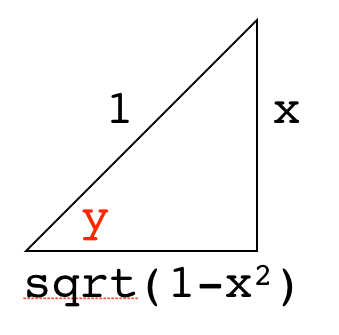
\includegraphics [scale=0.4] {arcsin3.png} \end{center}

\[ y = \sin^{-1}x \]
\[ \frac{dy}{dx} = ? \]

Write something we \emph{do} know
\[ x = \sin y \]
\[ \frac{dx}{dy} = \cos y \]
\[ \frac{dy}{dx} = \frac{1}{\cos y} = \frac{1}{\sqrt{1-x^2}} \]

Well alrighty then.  Now we just turn it into an integration problem:

\[ \int \frac{1}{\sqrt{1-x^2}}  \ dx = \sin^{-1} x + C \]

\subsection*{inverse tangent}

Visualize a different right triangle, again with $y$ as the angle, and $x$ as the side opposite but now $1$ is the side adjacent and $\sqrt{1+x^2}$ is the hypotenuse.

\[ y = \tan^{-1}x \]
\[ \frac{dy}{dx} = ? \]

And again, write something we \emph{do} know
\[ x = \tan y \]
\[ \frac{dx}{dy} = \sec^2 y \]
\[ \frac{dy}{dx} = \frac{1}{\sec^2 y} = \cos^2 y = \frac{1}{\sqrt{1+x^2}} \]

As before, we just turn it into an integration problem:

\[ \int \frac{1}{\sqrt{1+x^2}} \ dx = y = \tan^{-1}x + C\]

There is a simple relationship between inverse sine and cosine:

\[ \sin^{-1} x + \cos^{-1} = \frac{\pi}{2} \]
\[ \frac{d}{dx} \sin^{-1} x + \frac{d}{dx} \cos^{-1} = 0 \]
\[ \frac{d}{dx} \sin^{-1} x =  -  \frac{d}{dx} \cos^{-1}  \]
which is why we don't spend much time worrying about $\cos^{-1}$.

\subsection*{inverse secant}

The last useful one of these is the inverse secant.

We put $x$ as the hypotenuse, and $1$ as the side adjacent to the angle $y$.  Then the side opposite is $\sqrt{x^2-1}$.

\[ y = \sec^{-1} x \]
\[ \frac{dy}{dx} = ? \]

And yet again, write something we \emph{do} know
\[ x = \sec y \]
\[ \frac{dx}{dy} = \sec y \tan y  \]
\[ \frac{dy}{dx} = \frac{1}{\sec y} \ \frac{1}{ \tan y}  \]
\[ = \frac{1}{x} \ \frac{1}{\sqrt{x^2-1}} \]

Just turn it into an integration problem:

\[ \int \frac{1}{x \ \sqrt{x^2-1}}  \ dx = y = \sec^{-1}x + C\]

Examples 8 to 10 can all be re-written with a constant $a$ substituted for $1$.  In each case, the answer changes slightly (to have a function like $\tan^{-1}\frac{x}{a}$), and in the case of the last example, there is another factor of $1/a$ out in front.

One can handle these by re-drawing the triangle substituting $a$ for $1$, or one can factor the expression to obtain something like this:

\[ \int \frac{1}{\sqrt{a^2 - x^2}}  \ dx \]
\[ = \int \frac{1}{a} \ \frac{1}{\sqrt{1 - \frac{x^2}{a^2}}}  \ dx \]

Now substitute $t = x/a$ and $dt = dx/a$ so this is just
\[ = \int \ \frac{1}{\sqrt{1 - t^2} } \ dt \] 
\[ = \sin^{-1} t + C \]
\[ =  \sin^{-1} \frac{x}{a} + C \]

\end{document}  